\chapter{Design of the Two Controllers}
\label{ch:design}

This chapter specifies the two innovations at the level of signals, equations, and timing. Section~\ref{sec:visiondesign} designs the vision-guided feed-speed controller. Section~\ref{sec:mpcdesign} designs the multi-factor coordinator and the stack that joins the two. The hardware that gives these signals a physical place is specified in Section~\ref{sec:build}, after the signals are known, so that the build follows the information flow rather than the other way around.

\section{Vision-guided feed-speed control}
\label{sec:visiondesign}

\subsection{Role of the loop}

The feed-speed controller is a cascade with a constraint. The outer input is ground speed $v$ and the spacing set-point $X_t$. The inner output is a motor voltage, or a speed-mode torque command, that turns the cell wheel. Between them sits a scalar $\sigma\in[0.72,1.08]$ that multiplies the kinematic speed. When the throat looks clear, $\sigma$ stays near 1 and the loop is an ordinary electronic meter \cite{he2017,zhao2024}. When the throat looks bridged, $\sigma$ falls and the wheel waits. The waiting is the innovation. A tracker without the constraint would treat the same situation as a brief shortfall of fill and would not change its behaviour at all, because the shaft would still be at the commanded speed.

The loop does not detect species and does not draw boxes around seeds for an operator. It compresses each accepted frame into the features of Section~\ref{sec:features}. Those features are the only vision data the motor computer is allowed to see.

\subsection{Sensing and timing}

Two speed sensors are required by the problem set. A radar, or an encoder on an undriven wheel, supplies $v$. An encoder on the cell-wheel shaft supplies $\omega$. A driven ground wheel is logged and is not used in the control law, so that a later comparison with ground drive remains possible.

The camera looks down at the hopper throat through a window that is wiped mechanically. The region of interest is fixed in the image, about 640 by 200 pixels after cropping, covering the last few centimetres before the cell mouth. The exposure is strobed for 0.2~ms so that motion at 1.2~m/s does not smear a seed by more than a fraction of a millimetre at the working distance. The vision processor runs the steps of Section~\ref{sec:features} and publishes a feature datagram at 20~Hz. The motor computer runs at 100~Hz. If a datagram is late, the motor computer holds the previous bridge index and increments a miss counter. After three missed datagrams, 150~ms, it decays the bridge index by half each further period and the constraint opens. The motor never blocks on a frame. This split is the direct answer to the 6~km/h reversal reported when one microcontroller did both jobs \cite{borja2021}.

A photoelectric sensor in the seed tube is not inside the constraint. It is a logger. It counts releases so that an estimator can compare commanded rate with delivered rate. Using it as the bridge sensor would reintroduce the delay the camera is there to avoid \cite{kocher1998,lan1999}.

\begin{figure}[htbp]
\centering
\begin{tikzpicture}[
  font=\small,
  box/.style={draw, rounded corners=2pt, align=center, minimum height=8mm, inner sep=3pt},
  arr/.style={-{Stealth[length=2mm]}, thick}
]
\node[box] (cam) {Camera\\20~Hz};
\node[box, right=8mm of cam] (feat) {Features\\$d,\rho,B$};
\node[box, right=8mm of feat] (con) {Constraint\\$\sigma(B)$};
\node[box, below=12mm of con] (fuzzy) {Fuzzy PID\\100~Hz};
\node[box, left=8mm of fuzzy] (law) {Kinematic\\$\omega^{\star}$};
\node[box, left=8mm of law] (v) {Speed $v$};
\node[box, right=8mm of fuzzy] (mot) {Motor and\\cell wheel};
\node[box, below=11mm of mot] (enc) {Encoder $\omega$};
\draw[arr] (cam) -- (feat);
\draw[arr] (feat) -- (con);
\draw[arr] (con) -- (fuzzy);
\draw[arr] (v) -- (law);
\draw[arr] (law) -- (fuzzy);
\draw[arr] (fuzzy) -- (mot);
\draw[arr] (mot) -- (enc);
\draw[arr] (enc.west) -- ++(-8mm,0) |- (fuzzy.south);
\end{tikzpicture}
\caption{Vision features constrain the speed command. The motor loop closes on the encoder and does not wait for the camera.}
\label{fig:cascade}
\end{figure}

\subsection{Feature extraction}
\label{sec:features}

Each accepted gray frame is normalised by a running estimate of the empty-throat image, so that a slow change of dust does not move the threshold. Otsu's method then separates seed pixels from the background on the residual \cite{otsu1979,gonzalez2018}. Small components, below 20~mm$^2$ at the calibrated scale, are rejected as chips. The remaining components supply areas $A_j$ and perimeters. Equivalent diameters follow Equation~\eqref{eq:deq}. Occupancy is the seed-pixel area divided by the window area,
\begin{equation}
\rho = \frac{1}{A_{\mathrm{win}}}\sum_j A_j.
\label{eq:rho}
\end{equation}
The diameter summary used by the constraint is the mean $\bar d$ of the components and the coefficient of variation $c_d$ of those diameters. Circularity of component $j$ is
\begin{equation}
\gamma_j = \frac{4\pi A_j}{P_{\mathrm{er},j}^2}\in(0,1].
\label{eq:circ}
\end{equation}
An elongated acorn has a low $\gamma_j$. The bridge index combines occupancy, a circularity penalty, and oversize relative to the cell:
\begin{equation}
B = \rho\,(0.45 + 0.55\,\min(1, c_d/0.25))\,\Big(1 + \frac{\max(\bar d - d_c, 0)}{d_c}\Big).
\label{eq:bridge}
\end{equation}
The thresholds inside Equation~\eqref{eq:bridge} are design choices. Occupancy alone would treat a full but flowing throat as a bridge. The circularity term raises the index when the lot is irregular. The oversize term raises it when the seeds in view are larger than the 24~mm cell, which is the bur-oak situation. $B$ is dimensionless. In the numerical model the relief starts at $B>0.42$.

The same frame updates a one-pole filter that the constraint uses as its occupancy state,
\begin{equation}
\rho_{k+1} = 0.92\,\rho_k + 0.08\,\rho^{\mathrm{raw}}_k,
\label{eq:rhofilter}
\end{equation}
so that a single specular frame cannot slam the wheel. When the constraint is active and the wheel has slowed, the raw occupancy target inside the filter is pulled toward 0.48, representing a throat that is being allowed to clear. When the constraint is idle, the filter simply tracks the measurement.

\subsection{Kinematic command and the constraint}

With the nominal fill $\hat\eta=1$ and $N_c=12$,
\begin{equation}
\omega^{\star} = \frac{2\pi v}{12\, X_t}.
\label{eq:wstar2}
\end{equation}
At $v=1.10$~m/s and $X_t=0.25$~m, $\lambda^{\star}=4.40$~seeds/s and $\omega^{\star}=2.304$~rad/s, which is 22.0~r/min. At $v=0.70$~m/s the same spacing asks for 14.0~r/min. These are gentle shaft speeds. The motor is not being asked for maize peripheral speeds. It is being asked for a stable low speed under a changing load, which is a harder control problem than the raw number suggests, because stiction is a larger fraction of the torque.

The constrained command is
\begin{equation}
\omega_{\mathrm{cmd}} = \sigma(B)\,\omega^{\star},
\label{eq:wcmd}
\end{equation}
with
\begin{equation}
\sigma(B) =
\begin{cases}
1, & B \le 0.42,\\[4pt]
1 - \min\big(0.22,\ 0.55\,(B-0.42)\big), & B > 0.42.
\end{cases}
\label{eq:sigma}
\end{equation}
The largest cut is 22 percent. A bridge that would mathematically demand a stop is not allowed to stop the machine. The wheel keeps turning, the tube keeps receiving whatever seeds are free, and the index is recomputed. The lower clip at 0.72 and the upper clip at 1.08 are applied after $\sigma$ and after the small tracking residual of the inner loop, so a noisy fuzzy action cannot wind the scale outside that band.

Equation~\eqref{eq:sigma} is a static nonlinearity, not a second dynamic controller. Its stability effect is that it moves the setpoint. The inner loop is still asked to track a piecewise-constant speed. Setpoint moves are rate-limited at the equivalent of 8~rad/s$^2$ so that a newly detected bridge becomes a ramp rather than a step into the motor.

\subsection{Motor model}

The electrical and mechanical equations of a permanent-magnet direct-current motor, or of a current-controlled brushless motor reduced to the same form, are
\begin{align}
L\frac{\mathrm{d}i}{\mathrm{d}t} &= -Ri - K_e\omega + u, \label{eq:elec}\\
J\frac{\mathrm{d}\omega}{\mathrm{d}t} &= K_t i - b\omega - \tau_{\mathrm{load}}. \label{eq:mech}
\end{align}
The load torque $\tau_{\mathrm{load}}$ contains bearing friction, the intermittent torque of a seed entering a cell, and a stiction term that is largest when the hopper is full. For the speed loop the electrical pole is neglected. It sits well above 100~Hz on a small drive, and the current loop of a servo amplifier already hides it. The design model used for tuning is Equation~\eqref{eq:motor1}, repeated here with the numbers used in the estimation:
\begin{equation}
0.18\,\dot\omega + \omega = u_{\omega},
\label{eq:motornum}
\end{equation}
where $u_{\omega}$ is a speed command in the same units as $\omega$ after the inner current loop, and 0.18~s is the mechanical time constant under a representative hopper load. A 10~ms sample is twenty times faster than this pole, which is the usual rule for a discrete speed loop \cite{franklin2019,ogata2010}.

Load torque is not measured. It appears as a disturbance. Integral action rejects a constant disturbance. A seed that wedges and then releases is a pulse disturbance, which integral action handles if the gains are not so high that the pulse becomes an oscillation. The fuzzy layer exists to lower the proportional gain when the error is large and the error is still growing, and to raise it when the error is small, which is the standard reason for scheduling on a plant whose friction changes \cite{zhao2024,astrom2006}.

\subsection{Discrete fuzzy proportional--integral--derivative law}

Let the sample index of the motor loop be $n$, with $T_m=0.01$~s. The tracking error and its backward difference are
\begin{equation}
e_n = \omega_{\mathrm{cmd},n} - \omega_n, \qquad \Delta e_n = e_n - e_{n-1}.
\label{eq:err}
\end{equation}
The control law is
\begin{equation}
u_n = K_p(e_n,\Delta e_n)\, e_n + K_i(e_n,\Delta e_n)\, T_m\sum_{j=0}^{n} e_j + K_d(e_n,\Delta e_n)\,\frac{\Delta e_n}{T_m},
\label{eq:pid}
\end{equation}
with the integrator clamped and with the sum frozen whenever $|e_n|>e_{\mathrm{sep}}$. The separation threshold used here is $e_{\mathrm{sep}}=0.8$~rad/s. Integral separation is the device He and colleagues used to keep a large step from overshooting, and it is retained for the same reason \cite{he2017}. Anti-windup is the clamp: the summed error is not updated when $u_n$ is on its rail.

The gains are a nominal triple plus a bounded fuzzy increment,
\begin{equation}
K_p = K_{p0}+\Delta K_p,\quad
K_i = K_{i0}+\Delta K_i,\quad
K_d = K_{d0}+\Delta K_d,
\label{eq:gainsplit}
\end{equation}
with $K_{p0}=2.4$, $K_{i0}=6.0$, and $K_{d0}=0.08$ on the normalised speed model of Equation~\eqref{eq:motornum}. The increments are the outputs of a Mamdani inference on two inputs \cite{mamdani1974,zadeh1965}. Each input is scaled into the linguistic range by
\begin{equation}
\tilde e = \mathrm{sat}(e_n/0.6),\qquad \widetilde{\Delta e}=\mathrm{sat}(\Delta e_n/0.15),
\label{eq:scalee}
\end{equation}
where the saturation limits the argument to $[-1,1]$. The linguistic labels are negative big, negative small, zero, positive small, and positive big. Membership of the zero label is a triangle peaking at 0 with support $[-0.4,0.4]$. The small labels are triangles centred at $\pm 0.5$ with support of width 0.8. The big labels are trapezoids that reach membership 1 at $\pm 1$ and fall to 0 at $\pm 0.4$. The same shapes are used for both inputs. Figure~\ref{fig:member} draws the error membership. The increment memberships on the output universe $[-1,1]$ use the same five labels, and the inferred set is reduced to a number by the centroid.

\begin{figure}[htbp]
\centering
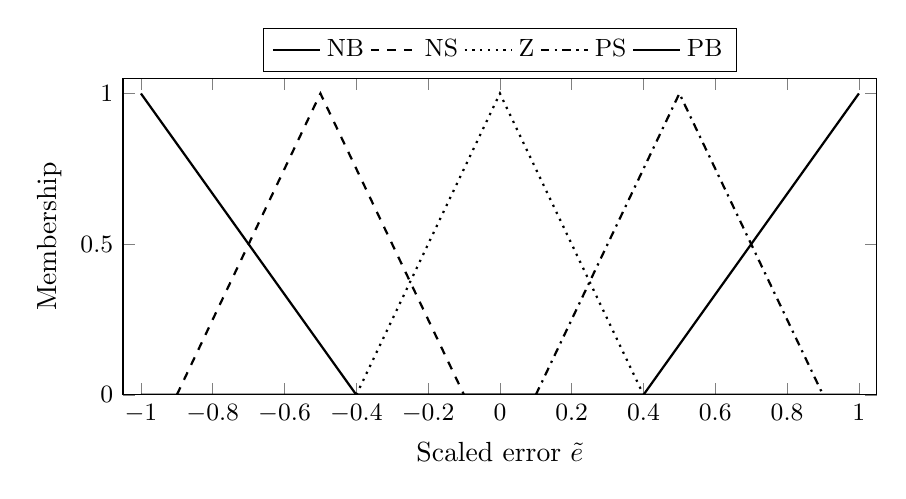
\begin{tikzpicture}
\begin{axis}[
  width=0.92\textwidth, height=5.6cm,
  xlabel={Scaled error $\tilde e$},
  ylabel={Membership},
  xmin=-1.05, xmax=1.05, ymin=0, ymax=1.05,
  legend style={font=\small, at={(0.5,1.02)}, anchor=south, legend columns=5},
  tick label style={font=\small}
]
\addplot[thick] coordinates {(-1,1) (-0.4,0) (1,0)};
\addlegendentry{NB}
\addplot[thick, dashed] coordinates {(-0.9,0) (-0.5,1) (-0.1,0)};
\addlegendentry{NS}
\addplot[thick, dotted] coordinates {(-0.4,0) (0,1) (0.4,0)};
\addlegendentry{Z}
\addplot[thick, dashdotted] coordinates {(0.1,0) (0.5,1) (0.9,0)};
\addlegendentry{PS}
\addplot[thick] coordinates {(-1,0) (0.4,0) (1,1)};
\addlegendentry{PB}
\end{axis}
\end{tikzpicture}
\caption{Membership of the scaled speed error. The same partition is used for the error increment. Output increments use the centroid of the fired labels.}
\label{fig:member}
\end{figure}

Table~\ref{tab:fuzzy} lists the rule for $\Delta K_p$. The rules for $\Delta K_i$ use the opposite corner emphasis: integral gain is allowed to rise only when both the error and the increment are near zero, and it is cut when the error is large, which keeps the separator and the fuzzy layer from fighting. The rules for $\Delta K_d$ raise derivative gain when the error and the increment have the same sign and a large magnitude, that is, when the shaft is running away from the command. Rules are written in the usual condensed form. ``Error is negative big and the increment is negative big implies $\Delta K_p$ positive big'' means the loop is below the command and still falling, so proportional action should strengthen.

\begin{table}[htbp]
\centering
\caption{Rule table for the proportional increment $\Delta K_p$. Rows are the scaled error. Columns are the scaled error increment.}
\label{tab:fuzzy}
\begin{tabular}{@{}lccccc@{}}
\toprule
 & NB & NS & Z & PS & PB \\
\midrule
NB & PB & PB & PS & Z & NS \\
NS & PB & PS & PS & Z & NS \\
Z & PS & PS & Z & NS & NS \\
PS & PS & Z & NS & NS & NB \\
PB & Z & NS & NS & NB & NB \\
\bottomrule
\end{tabular}
\end{table}

The centroid is scaled into the increments by $\Delta K_p \in [-0.8, 0.8]$, $\Delta K_i \in [-2, 2]$, and $\Delta K_d \in [-0.03, 0.03]$. These boxes are part of the design. At every corner, $K_p$ and $K_i$ stay positive, so the proportional--integral polynomial of Equation~\eqref{eq:pi-char} keeps positive coefficients on the design model. A pure derivative $K_d s$ is improper on Equation~\eqref{eq:motornum}. The implementation filters the difference with a first-order pole at 40~Hz, which keeps the high-frequency gain finite \cite{astrom2006}. The resulting claim is limited on purpose. Positive frozen gains and a filtered derivative make each frozen loop a standard stable speed servo on Equation~\eqref{eq:motornum}. They are not a Lyapunov certificate for the time-varying fuzzy system \cite{khalil2002}. The schedule is still reasonable because it moves with the tracking error, and the error of a 0.18~s plant does not cross the whole linguistic range in one 10~ms sample unless the setpoint jumps. Setpoint jumps are rate-limited, as already stated. A vertex check of the discrete spectral radius belongs to the implementation test of a future build. It is not reported as a completed numerical proof in this manuscript.

\subsection{What the constraint does to a spacing sequence}

A cell event occurs every time the wheel advances by $2\pi/N_c$. If the scale $\sigma$ is constant over the event, the distance the machine travels between events is
\begin{equation}
\Delta x = \frac{v}{\lambda} = \frac{X_t}{\sigma},
\label{eq:deltax}
\end{equation}
because $\lambda=\sigma v/X_t$ when the fill is one seed per event. A scale of 0.85 stretches the geometric spacing by $1/0.85\approx 1.18$. Part of that stretch is the point of the constraint: a double that would have produced a 0.2$X_t$ gap is replaced by a later single. Part of the stretch is a new miss if the following event is empty for an unrelated reason. The estimation has to be able to show both parts. A controller that is scored only on doubles will always want the lowest $\sigma$. The efficiency index of Equation~\eqref{eq:eta} punishes the stretch.

The photoelectric count provides a runtime estimate of fill after the fact,
\begin{equation}
\hat\eta_{n} = \frac{N_{\mathrm{tube}}(t_n)-N_{\mathrm{tube}}(t_n-T_{\eta})}{N_c\,(\theta(t_n)-\theta(t_n-T_{\eta}))/2\pi},
\label{eq:etahat}
\end{equation}
with $T_{\eta}=2$~s. This estimate is logged. It is not allowed to divide Equation~\eqref{eq:wstar2} in the present design. Dividing by a noisy $\hat\eta$ rebuilds the kinematic command every two seconds and fights the constraint. A later revision can blend $\hat\eta$ into $\omega^{\star}$ with a time constant of tens of seconds, once a bench has shown that the estimate is calm. The requirement list does not demand that blend.

\subsection{Worked numbers for a red-oak frame}

Take a red-oak mean diameter of 20.5~mm, a lot coefficient of variation of 0.15, and a cell of 24~mm. Suppose the filtered occupancy is 0.62. Equation~\eqref{eq:bridge} gives
\begin{equation}
B = 0.62\,(0.45+0.55\cdot 0.15/0.25)\,(1+0) = 0.62\cdot 0.78 = 0.484,
\end{equation}
because $c_d/0.25=0.60$ and there is no oversize. The excess over 0.42 is 0.064, and $0.55\times 0.064=0.035$, which is below the 0.22 cap. The scale drops from 1 to 0.965. At 1.10~m/s the commanded shaft speed falls from 22.0~r/min to 21.2~r/min. The intervention is small because this frame is only mildly occupied and the seeds fit the cell. That is the correct behaviour. The constraint is not a permanent detune.

Now take a bur-oak frame with $\bar d=32$~mm, $c_d=0.20$, and $\rho=0.70$. Then
\begin{equation}
B = 0.70\,(0.45+0.55\cdot 0.80)\,\big(1+(32-24)/24\big) = 0.70\cdot 0.89\cdot 1.333 = 0.830.
\end{equation}
The excess is 0.410, and $0.55\times 0.410=0.226$, which the cap cuts to 0.22. The scale is 0.78, and the shaft command falls from 22.0~r/min to 17.2~r/min. The wheel gives the large seeds more time. Whether that time becomes filled cells or merely larger gaps is decided by the vibrator as well as by the wheel, which is why the second loop exists. Vision alone, in the later tables, improves doubles more reliably than it improves misses.

\subsection{Fault states inside the feed loop}

Four fault states are defined so that the real-time program has somewhere to go.

\begin{enumerate}
\item \textbf{Vision hold.} A late datagram holds $B$. Tracking continues. A counter is incremented.
\item \textbf{Vision decay.} After 150~ms, $B$ is halved each 50~ms until it lies below 0.42. The constraint opens. The operator lamp for vision is lit. The motor loop is unchanged.
\item \textbf{Encoder loss.} If the shaft encoder misses two periods, the motor current is removed and the wheel stops. Coasting a cell wheel with an unknown speed is how doubles become a pile. This state is a stop, not a fallback to open voltage.
\item \textbf{Speed-sensor loss.} If $v$ is stale for 200~ms, $\omega^{\star}$ is held at its last value for 1~s and then ramped to zero. Holding forever would keep planting after the tractor has stopped only if the failure mode is a stuck high reading, which is unsafe. Ramping down is the chosen failure direction.
\end{enumerate}

None of these states requires the factor coordinator. They are local to the feed computer. The factor computer is informed by a single health bit so that it can freeze $u$ when the wheel is stopped, rather than integrating a model that assumes events are still occurring.

\section{Multi-factor model-predictive optimization}
\label{sec:mpcdesign}

\subsection{Role of the loop}

The factor coordinator owns vibration frequency $f$, assist vacuum $P$, and opener depth $h$. It does not own the wheel speed. It runs at 5~Hz, which is once every 200~ms, and on this machine that is once every few cell events at the speeds of interest. Its job is to keep the triple $(f,P,h)$ at a point where the fast loop's constraint is rarely needed. A coordinator that needs the constraint to look good has chosen a bad regime. For that reason the prediction inside the coordinator is evaluated at $\sigma=1$ and with the vision flag clear. The vision loop may still act, and the estimation credits that action separately. The coordinator is not allowed to assume that the action will happen.

This separation is also a software separation. The factor task can overrun a deadline without stretching a motor period. On an overrun the previous feasible triple is held. Holding a feasible input is the standard fallback of a predictive controller that misses a sample \cite{maciejowski2002,rawlings2017}.

\subsection{Prediction model}
\label{sec:predmodel}

The model is a logistic map from a seed diameter and a factor triple to the probabilities of a miss and a double at one cell event. It is the map $\Pi$ of Equation~\eqref{eq:pi}, written so that it can be evaluated inside a grid search. Define the normalised size errors and the harshness of the motion that the seed mass actually feels:
\begin{align}
\delta_{+} &= \max(d-d_c,0)/d_c, &
\delta_{-} &= \max(d_c-d,0)/d_c, \label{eq:delta}\\
f^{\star}(d) &= \mathrm{clip}\big(4 + 5\, d_c/d,\ 3,\ 11\big), \label{eq:fstar}\\
a(f,d) &= \exp\Big(-\big((f-f^{\star}(d))/2.6\big)^2\Big), \label{eq:agit}\\
H(f_{\mathrm{eff}}) &= \max(f_{\mathrm{eff}}-10, 0)/10. \label{eq:harsh}
\end{align}
The preferred frequency $f^{\star}$ falls as the seed gets larger: a 32~mm seed prefers about 7.8~Hz before the clip, and a 15~mm seed prefers about 12~Hz before the clip, which then limits it to 11~Hz. The Gaussian $a$ is near 1 only when the command sits close to that preference. Harshness $H$ is zero at or below the 10~Hz anchor taken from the rapeseed vibration trials and rises linearly above it \cite{zhang2024vib}. The frequency that enters $H$ is not the command alone. Terrain and the shaker both reach the box,
\begin{equation}
f_{\mathrm{eff}} = \sqrt{\big(\alpha_{\mathrm{iso}} f_{\mathrm{dist}}\big)^2 + f^2}.
\label{eq:feff}
\end{equation}
When the coordinator is off, the isolator is treated as passive and $\alpha_{\mathrm{iso}}=1$. When the coordinator is on, the mount described in Section~\ref{sec:build} is taken to attenuate the terrain contribution to $\alpha_{\mathrm{iso}}=0.55$. That number is an assumption of the model, not a measured transmissibility. It is applied consistently in the estimation, and the text that discusses energy will show what the assumption does: the optimiser can park $f_{\mathrm{eff}}$ just under 10~Hz by a combination of isolation and a modest command.

Depth error, slip, and speed-scale error enter as further dimensionless terms,
\begin{equation}
\varepsilon_h = |h-h^{\star}|/h^{\star},\qquad
o_{\sigma}=\max(\sigma-1.08,0),\qquad
u_{\sigma}=\max(0.92-\sigma,0),
\label{eq:errs}
\end{equation}
with $h^{\star}=30$~mm. The linear predictors are
\begin{align}
\begin{split}
z_m ={}& -1.55 + 5.2\,\delta_{+} + 2.4\,H + 2.6\,s + 2.2\,o_{\sigma} + 1.4\,u_{\sigma} \\
&+ 1.3\,\varepsilon_h - 1.7\,a\,(0.35+\delta_{+}) - 0.85\,\nu\, a,
\end{split} \label{eq:zm}\\
\begin{split}
z_d ={}& -2.05 + 3.6\,\delta_{-} + 1.7\,(P/8)\,(0.4+\delta_{-}) \\
&+ 1.1\,\frac{\max(6-f,0)}{6}\,\delta_{-} + 0.6\,o_{\sigma} - 0.9\,\nu - 0.5\,a.
\end{split} \label{eq:zd}
\end{align}
Here $\nu\in\{0,1\}$ is the vision flag, which the coordinator sets to 0. The probabilities are
\begin{equation}
p_m = \ell(z_m),\qquad
p_d = \ell(z_d)\,(1-p_m),\qquad
p_s = 1-p_m-p_d,
\label{eq:probs}
\end{equation}
with the logistic function $\ell(z)=(1+e^{-z})^{-1}$ evaluated on a clipped $z$ so that the implementation cannot overflow. Scatter of a qualified spacing is modelled as a standard deviation
\begin{equation}
\begin{split}
\varsigma = X_t\Big(&0.07 + 0.045\,H + 0.035\,\varepsilon_h + 0.03\,|\sigma-1| \\
&+ 0.02\,(1-0.6\nu) + 0.015\,|f-f^{\star}|/6\Big).
\end{split}
\label{eq:sigma_scatter}
\end{equation}
Equation~\eqref{eq:sigma_scatter} does not feed the logistic. It feeds the cost, as a stand-in for the precision term.

Each coefficient has a stated job. The intercepts $-1.55$ and $-2.05$ set a mild baseline miss and double probability when every error term is zero and agitation is absent: $\ell(-1.55)\approx 0.175$ and $\ell(-2.05)\approx 0.114$ before the agitation credit, which is then modified by $a$. The large coefficient 5.2 on $\delta_{+}$ is the Wells effect, written as a steep miss penalty once the seed exceeds the cell \cite{wells1990}. The coefficient 3.6 on $\delta_{-}$ is the double penalty for a small seed in a large cell \cite{yazgi2007,onal2012}. The vacuum term is multiplied by $(0.4+\delta_{-})$ so that vacuum is almost harmless when the seed fills the cell and is harmful when the seed is small. The harshness coefficient 2.4 is the Zhang effect, scaled so that a disturbance well above 10~Hz moves the miss probability by tens of points if isolation is absent \cite{zhang2024vib}. None of these coefficients was fitted to a new data set. Replacing them with fitted values is future experimental work. Keeping them public is what makes Chapter~\ref{ch:estimate} repeatable.

\subsection{A numerical evaluation of the map}

The map should be evaluated once by hand so that the later tables have an anchor. Consider red oak at $d=20.5$~mm, $d_c=24$~mm, so $\delta_{+}=0$ and $\delta_{-}=3.5/24=0.1458$. The preferred frequency is
\begin{equation}
f^{\star} = 4 + 5\cdot(24/20.5) = 9.85~\text{Hz},
\end{equation}
inside the clip. With a command $f=9$~Hz,
\begin{equation}
a = \exp\big(-((9-9.85)/2.6)^2\big) = \exp(-0.107) = 0.899.
\end{equation}
Under the coordinator, a terrain frequency of 6~Hz and $\alpha_{\mathrm{iso}}=0.55$ give
\begin{equation}
f_{\mathrm{eff}} = \sqrt{(0.55\cdot 6)^2 + 9^2} = \sqrt{91.89} = 9.59~\text{Hz},
\end{equation}
so $H=0$. Take $\sigma=1$, $s=0.004$, $\varepsilon_h=0$, and $\nu=1$ for a feed-loop evaluation (the coordinator itself would set $\nu=0$). Then
\begin{align}
z_m &= -1.55 + 2.6\cdot 0.004 - 1.7\cdot 0.899\cdot 0.35 - 0.85\cdot 0.899 \nonumber\\
&= -1.55 + 0.010 - 0.535 - 0.764 = -2.84,\\
p_m &= \ell(-2.84) = 0.055.
\end{align}
The double predictor with $P=0$ is
\begin{align}
z_d &= -2.05 + 3.6\cdot 0.1458 - 0.9 - 0.5\cdot 0.899 \nonumber\\
&= -2.05 + 0.525 - 0.9 - 0.450 = -2.87,\\
p_d &= \ell(-2.87)\,(1-0.055) = 0.054\cdot 0.945 = 0.051.
\end{align}
About 89 percent of events at this single diameter are singles before spacing classification. The quality-of-feed index in a full Monte Carlo run is lower than this event-single rate, because spacing classification also punishes rate error, but the event rate shows that the stacked loops sit in a high-single region for a seed that fits the cell.

The contrasting ground-drive evaluation uses $f=0$, $P=3$~kPa, $\nu=0$, $s=0.07$, $\sigma=0.93$, and $f_{\mathrm{eff}}=6$ so that $H=0$. Agitation $a$ is essentially zero because the command is many standard deviations from 9.85~Hz. Then $z_m=-1.55+2.6\cdot 0.07=-1.37$ and $p_m=\ell(-1.37)=0.203$. The double predictor picks up both the size term and the vacuum term,
\begin{equation}
z_d = -2.05 + 0.525 + 1.7\cdot(3/8)\cdot 0.546 + 1.1\cdot 0.146 = -1.02,
\end{equation}
so $\ell(z_d)=0.266$ and $p_d=0.266\cdot(1-0.203)=0.212$. The event-single probability is about 0.58. The ground-drive rows in Chapter~\ref{ch:estimate} land on a quality-of-feed index of the same order. The map is doing what it was constructed to do: a fitted cell without agitation and with a few kilopascals of vacuum doubles a slightly small seed, and wheel slip adds misses.

\subsection{Cost and constraints}

At a coordinator step the diameter distribution is represented by three points, the running mean $\bar d$, the high point $\bar d(1+c_d)$, and the low point $\bar d(1-c_d)$, with weights $1/2$, $1/4$, and $1/4$. The running mean is the vision mean when vision is healthy and a hopper-sample mean entered by the operator otherwise. Using three points rather than a full quadrature is a load decision. The factor computer must finish inside 200~ms with margin, and three evaluations of $\ell$ are cheap.

The cost summed over the three points is
\begin{equation}
J(f,P,h) = \sum_{i=1}^{3} w_i\Big(9\, p_m^{(i)} + 6\, p_d^{(i)} + 4\,\varsigma^{(i)}/X_t + 0.004\, f + 0.01\, P\Big),
\label{eq:cost}
\end{equation}
with $\sigma=1$, $\nu=0$, and the slip inside the prediction fixed at 0.02 because the electronic drive, not the coordinator, is responsible for slip. Depth is not searched. The depth servo is required to hold $h^{\star}$, and the prediction uses $h=h^{\star}$. Searching depth as well would only restate that the best depth error is zero. The servo's value appears in the estimation as a reduction of the depth noise, from a standard deviation of 6.5~mm with a passive opener to 1.2~mm with the servo. That reduction changes $\varepsilon_h$ in Equation~\eqref{eq:zm} and is part of the second innovation's hardware, not a third control algorithm.

The searched set is the Cartesian product
\begin{equation}
f\in\{2,3,\ldots,12\}~\text{Hz by steps of 1},\qquad
P\in\{0, 1, 2, 3.5, 5\}~\text{kPa}.
\label{eq:grid}
\end{equation}
Eleven frequencies and five pressures give 55 costs. Each cost is three logistic evaluations. The search is exhaustive on this set, so the computed minimiser is exact on the set. Exhaustive search on 55 points is a model-predictive controller whose horizon is one statistical step and whose input set is a grid. It is not a long-horizon quadratic program. It is still receding-horizon control in the original sense: the first, and only, move of the solved problem is applied, and the problem is solved again at the next sample with updated $\bar d$ and $f_{\mathrm{dist}}$ \cite{garcia1989,clarke1987}. A one-step horizon is justified because the factor commands have no meaningful dynamics inside 200~ms other than actuator lag, and the lag is handled by a slew limit rather than by a multi-step model. Frequency may change by at most 2~Hz per sample. Vacuum may change by at most 1~kPa per sample. The opener servo has its own loop and is not slewed by this search.

The prices 0.004 on frequency and 0.01 on vacuum are small next to a miss probability of 0.2, which is multiplied by 9. They matter when two grid points have almost the same predicted misses. In that flat region the optimiser prefers the quieter point. Under a harsh terrain disturbance the flat region is not where the action is: adding shaker frequency raises $f_{\mathrm{eff}}$ through Equation~\eqref{eq:feff} and can push $H$ above zero. The price and the harshness term then agree, and the command falls. The estimation shows this fall, from 9~Hz in a mild case to 3~Hz when $f_{\mathrm{dist}}=16$~Hz.

\begin{figure}[htbp]
\centering
\begin{tikzpicture}[
  font=\small,
  box/.style={draw, rounded corners=2pt, align=center, inner sep=3pt, minimum width=32mm},
  arr/.style={-{Stealth[length=2mm]}, thick}
]
\node[box] (meas) {Measurements\\$\bar d, c_d, f_{\mathrm{dist}}$};
\node[box, below=11mm of meas] (pred) {Logistic map\\$\nu=0$, $\sigma=1$};
\node[box, below=11mm of pred] (grid) {55-point grid\\$\min J(f,P)$};
\node[box, below=11mm of grid] (slew) {Slew limit\\hold last if late};
\node[box, right=16mm of slew] (act) {Shaker, vacuum\\regulator, depth servo};
\node[box, right=16mm of pred] (fast) {Feed loop\\uses $\nu=1$\\and its own $\sigma(B)$};
\draw[arr] (meas) -- (pred);
\draw[arr] (pred) -- (grid);
\draw[arr] (grid) -- (slew);
\draw[arr] (slew) -- (act);
\draw[arr] (meas.east) -- ++(8mm,0) |- (fast.north);
\draw[arr] (fast.south) -- ++(0,-28mm) -| (act.north);
\end{tikzpicture}
\caption{The factor search predicts the meter with vision off. The feed loop then applies the bridge constraint on top of the chosen factors. Neither loop waits for the other.}
\label{fig:hierarchy}
\end{figure}

\subsection{Relation to a quadratic program}

A reader who expects the classical quadratic program can recover it as an approximation. Let $x$ stack the three probabilities and the normalised scatter at the mean diameter, and let the grid be replaced by a box $u\in\mathcal U$. Linearising $\Pi$ about the previous command $u^{-}$ gives
\begin{equation}
x \approx x^{-} + G\,(u-u^{-}),
\label{eq:lin}
\end{equation}
and the cost $9p_m+6p_d+4\varsigma/X_t$ plus a move penalty $(u-u^{-})^{\mathsf T} R (u-u^{-})$ is a convex quadratic if one ignores the logistic curvature, or if one keeps the curvature and accepts a sequential quadratic program \cite{nocedal2006,boyd2004}. Constraints are the box and the slew. That program is the form surveyed by Qin and Badgwell and analysed by Mayne and colleagues \cite{qin2003,mayne2000}. It was not the form implemented for the estimation, because the logistic is cheap to evaluate exactly and the input dimension is two once depth is removed. The grid avoids a linearisation error near $\delta_{+}=0$, where the $\max(\cdot,0)$ terms are not differentiable and a gradient method needs a subgradient convention.

An explicit multi-parametric solution in the sense of Bemporad and colleagues would be attractive if the linear model were trusted, because the control law would become a lookup of critical regions \cite{bemporad2002}. With a non-smooth logistic and an input grid of 55 points, the lookup is the grid itself. Memory on the factor computer is not the binding constraint. Deadline margin is. Fifty-five evaluations leave the processor idle for most of the 200~ms period, which is the desired state of a safety-related task: busy for a short, bounded time, then waiting.

Stability of a one-step constrained search on a static map is simpler than stability of a dynamic horizon. The applied $u$ is always one of the 55 feasible points, the slew limit makes the applied sequence Lipschitz in time, and the plant-side actuators are themselves stable servos. There is no hidden unstable mode in the coordinator. The quality of the closed loop is entirely a question of whether $J$ ranks the true probabilities in the right order. That is a model-quality question, and Chapter~\ref{ch:estimate} does not answer it experimentally. It answers the narrower question of how the indices move when the plant is the same map the coordinator optimises, with Monte Carlo variation of diameter, slip, and depth noise that the coordinator does not see seed by seed. Even in that favourable situation the coordinator is not given the per-seed diameter, only the lot statistics, so the comparison is not a tautology of perfect preview.

\subsection{Information the coordinator is denied}

The following quantities are measured somewhere on the machine and are intentionally not inputs to $J$.

\begin{enumerate}
\item The instantaneous bridge index $B$. If $J$ could see $B$, it would learn to leave a bridge in place and let $\sigma(B)$ clean it up, which shows up as good $p_d$ in a joint predictor and as a poor $\eta_{\mathrm{E}}$ on the machine.
\item The tube count over the last second. That count is the outcome. Using it inside the same period double-counts the event the cost is predicting. A slow outer trim of the intercepts in Equations~\eqref{eq:zm} and \eqref{eq:zd}, with a time constant of a minute, is a reasonable adaptive extension \cite{ljung1999,kalman1960,welch1995}. It is not part of this design.
\item Opener draft force. Draft is a useful depth-loop measurement and a poor miss predictor unless it is calibrated per soil. The depth loop closes on a potentiometer. Draft is logged for a future soil-specific correction.
\end{enumerate}

Denying information is part of the architecture. A hierarchical controller that passes every measurement to every layer becomes a single optimiser with a distributed implementation, and it fails as a single optimiser \cite{skogestad2005}. The bit that does pass upward is health: vision alive, encoder alive, wheel stopped. Health bits change modes. They do not enter $J$ as if they were diameters.

\subsection{Stacking the loops}

The stack at a moment when both loops are healthy is the following sequence. The description is the program order on two computers that share a small datagram and do not share a clock beyond a 1~ms time stamp.

\begin{enumerate}
\item The vision computer publishes $\bar d$, $c_d$, $\rho$, and $B$.
\item The factor computer, if it is on a 200~ms boundary, reads $\bar d$, $c_d$, and the latest inertial estimate of $f_{\mathrm{dist}}$, evaluates $J$ on the grid with $\nu=0$, slew-limits the winner, and publishes $(f,P)$. The depth servo is continuously commanded to $h^{\star}$ and does not wait for this boundary.
\item The motor computer reads $v$ and $B$, forms $\omega_{\mathrm{cmd}}$ from Equations~\eqref{eq:wstar2}--\eqref{eq:sigma}, and runs Equation~\eqref{eq:pid} at 100~Hz.
\item The shaker amplifier and the vacuum regulator track $f$ and $P$ with their own current loops. Those loops are not redesigned here. They are required to reach a 2~Hz step in under 150~ms and a 1~kPa step in under 150~ms, which is the slew assumption made above.
\end{enumerate}

Interference, if it appears, will appear as a gain in $Q_{\mathrm{f}}$ that does not appear in $\eta_{\mathrm{E}}$, because $\sigma<1$ stretches spacings. The problem statement asked for that distinction to be preserved in the report. The estimation therefore publishes both indices for every case, including the cases where vision alone lowers efficiency relative to a pure speed loop. That outcome is a successful warning from the design, not a failure of the table.

\subsection{Parameter summary}

Table~\ref{tab:params} collects the numbers a reimplementation needs. Anything not in the table is a logging choice and does not change the indices.

\begin{table}[htbp]
\centering
\caption{Design parameters used by both the controllers and the numerical estimation.}
\label{tab:params}
\begin{tabular}{@{}llr@{}}
\toprule
Symbol & Role & Value \\
\midrule
$X_t$ & Target spacing & 0.25~m \\
$N_c$ & Cells on the wheel & 12 \\
$d_c$ & Cell mouth & 24~mm \\
$h^{\star}$ & Target depth & 30~mm \\
$T_m$ & Motor period & 10~ms \\
$T_v$ & Vision period & 50~ms \\
$T_f$ & Factor period & 200~ms \\
$\tau$ & Motor time constant & 0.18~s \\
$B_{\mathrm{on}}$ & Constraint threshold & 0.42 \\
$\sigma_{\min}$ & Deepest feed cut & 0.78 \\
$K_{p0},K_{i0},K_{d0}$ & Nominal gains & 2.4,\ 6.0,\ 0.08 \\
$\alpha_{\mathrm{iso}}$ & Terrain attenuation, coordinator on & 0.55 \\
$f_{\mathrm{harsh}}$ & Harshness anchor & 10~Hz \\
Grid & Frequency and vacuum & 11 by 5 points \\
Weights & $p_m$, $p_d$, $\varsigma/X_t$ & 9,\ 6,\ 4 \\
Prices & Per hertz and per kilopascal & 0.004,\ 0.01 \\
\bottomrule
\end{tabular}
\end{table}

The two innovations are now fully specified as programs. The rest of this chapter records the discrete realization, one fully numerical inference, the flight of a seed after release, the schedulability argument, and a slice of the cost grid. The next chapter places the programs on a machine and runs them under the lots and disturbances of the problem set.

\subsection{Discrete realization of the speed loop}
\label{sec:discrete}

Equation~\eqref{eq:motornum} is continuous. The feed computer is not. With a zero-order hold on the command and a sample $T_m=0.01$~s, the exact discretization of $\tau\dot\omega+\omega=u_{\omega}$ is a first-order difference
\begin{equation}
\omega_{n+1} = a\,\omega_n + (1-a)\,u_n, \qquad a = e^{-T_m/\tau}.
\label{eq:discplant}
\end{equation}
Substituting $\tau=0.18$~s gives $T_m/\tau=0.0556$ and $a=0.9460$. The one-step gain on the command is $1-a=0.0540$. A command that steps by 1~rad/s therefore moves the shaft by only 0.054~rad/s on the next sample, which is why the loop needs many samples to finish a bridge-induced ramp and why a 10~ms budget is comfortable for the arithmetic even though it is tight for a stall detector.

The proportional--integral law without the derivative, written backwards in time so that it can be coded as a recurrence, uses the summed error $s_n$ and the clamped increment
\begin{equation}
s_n =
\begin{cases}
s_{n-1}, & |e_n|>0.8~\text{rad/s or } u \text{ on its rail},\\
s_{n-1}+T_m e_n, & \text{otherwise},
\end{cases}
\label{eq:sum}
\end{equation}
and
\begin{equation}
u_n = \mathrm{sat}\big(K_p e_n + K_i s_n + K_d\,\delta_n\big),
\label{eq:usat}
\end{equation}
where $\delta_n$ is the filtered difference. The derivative filter is itself a discrete pole. A continuous pole at 40~Hz has time constant $1/(2\pi\cdot 40)\approx 4.0$~ms. Its exact sample coefficient at 10~ms is not the right object, because the difference is already a once-per-sample quantity. The implementation uses an exponential smoother on $\Delta e_n/T_m$,
\begin{equation}
\delta_n = \beta\,\delta_{n-1} + (1-\beta)\,\frac{e_n-e_{n-1}}{T_m}, \qquad \beta = e^{-T_m/\tau_d},
\label{eq:dfilt}
\end{equation}
with $\tau_d=4$~ms, so $\beta=e^{-2.5}=0.0821$. The filter is fast relative to the motor and slow relative to a single-sample encoder spike. An encoder that glitches by one count on a 4096-count wheel at 22~r/min produces a false $\Delta\omega$ of $2\pi/4096$ radians in 10~ms, which is 0.15~rad/s of false rate. Multiplied by $K_d=0.08$ that glitch is a 0.012~rad/s command bump, smaller than the tracking residual already budgeted in the estimation. The filter is what keeps a two-count glitch from becoming a command. This arithmetic is the sort of check that belongs in the feed computer's design review. It is not a result from a logic analyser.

Integral separation and the rail clamp interact. If the clamp freezes $s_n$ while the separation condition is also true, the sum is frozen once, not twice. The code path must be a single conditional. Two nested conditionals that both subtract the last addition will drift. The specification is Equation~\eqref{eq:sum}: one freeze flag, the logical or of the two reasons.

\subsection{A numerical fuzzy step}

The rule table is easier to trust after one sample is evaluated by hand. Take $e_n=0.30$~rad/s and $e_{n-1}=0.35$~rad/s, so the shaft is below the command and the error is shrinking. The scaled inputs of Equation~\eqref{eq:scalee} are
\begin{equation}
\tilde e = 0.30/0.6 = 0.50, \qquad \widetilde{\Delta e} = (0.30-0.35)/0.15 = -0.333.
\end{equation}
On the error partition of Figure~\ref{fig:member}, $\tilde e=0.50$ sits on the peak of the positive-small triangle, so $\mu_{\mathrm{PS}}(\tilde e)=1$. The positive-big trapezoid is 0 at 0.4 and 1 at 1.0, so
\begin{equation}
\mu_{\mathrm{PB}}(\tilde e) = (0.50-0.40)/(1.00-0.40) = 0.167.
\end{equation}
Zero, negative-small, and negative-big are 0 at this point. On the increment, $-0.333$ falls inside the negative-small triangle centred at $-0.5$ with support from $-0.9$ to $-0.1$. The left slope would be irrelevant. The right slope runs from membership 1 at $-0.5$ to 0 at $-0.1$, and $-0.333$ is $(0.5-0.333)/0.4=0.417$ of the way from the centre to the edge, so $\mu_{\mathrm{NS}}(\widetilde{\Delta e})=1-0.417=0.583$. The zero triangle has support $[-0.4,0.4]$ and peak 1 at 0, so at $-0.333$ its membership is $1-0.333/0.4=0.168$. Negative-big is the trapezoid that is 1 at $-1$ and 0 at $-0.4$. At $-0.333$ it is already 0.

Four rule conjunctions survive, using the minimum for ``and''. From Table~\ref{tab:fuzzy}, error positive-small and increment negative-small fires $\Delta K_p$ at label Z with strength $\min(1,0.583)=0.583$. Error positive-small and increment zero fires NS with strength $\min(1,0.168)=0.168$. Error positive-big and increment negative-small fires NS with strength $\min(0.167,0.583)=0.167$. Error positive-big and increment zero fires NS with strength $\min(0.167,0.168)=0.167$. The output labels are placed at Z$=0$ and NS$=-0.5$ on the increment universe. Aggregating by the maximum, the Z spike has height 0.583 and the NS spike has height $\max(0.168,0.167,0.167)=0.168$. A centroid of two spikes is
\begin{equation}
c = \frac{0.583\cdot 0 + 0.168\cdot(-0.5)}{0.583+0.168} = -0.112.
\end{equation}
Scaled into the proportional box $[-0.8,0.8]$, the increment is $\Delta K_p=-0.090$. The nominal $K_{p0}=2.4$ becomes $K_p=2.31$. The loop is close to the command and the error is already shrinking, so the scheduler slightly reduces proportional gain rather than kicking the shaft. A large growing error would have fired the PB corner of the table and moved $\Delta K_p$ the other way. The example is the ordinary sample, which is the sample the machine sees most often. A design that only behaves well on the linguistic corners and chatters in the middle is the design this calculation is meant to forbid.

The same sample's integral rules, which cut $K_i$ away from zero error, produce a small negative $\Delta K_i$ because $\tilde e$ is not inside the zero label. Derivative rules see an error and an increment of opposite signs, so they do not raise $K_d$. The net command correction relative to the nominal triple is a few percent. That is what ``bounded schedule'' means in a number rather than in a slogan \cite{mamdani1974,takagi1985}.

\subsection{Flight after release}
\label{sec:flight}

The spacing model in the estimation advances the tractor by $X_t/\sigma$ and then adds a random scatter. The scatter has a mechanical source that should be written down so a bench can look for it. A seed leaves the cell at angle $\psi$ below the horizontal with speed $r\omega$ relative to the housing, and the housing moves at $v$. In a frame fixed to the ground at the release instant the initial velocity is
\begin{equation}
\dot x(0) = v - r\omega\cos\psi, \qquad \dot y(0) = -r\omega\sin\psi,
\label{eq:v0}
\end{equation}
with $y$ positive upward and the tube entrance a distance $L_t$ below the release. For the nominal wheel, $r=0.09$~m and $\omega=2.30$~rad/s, so $r\omega=0.207$~m/s. At $\psi=70^\circ$, which is a release on the lower rear of the wheel, $\dot x(0)=v-0.071$~m/s and $\dot y(0)=-0.195$~m/s. The time to fall $L_t=0.40$~m under gravity, ignoring wall strikes, solves
\begin{equation}
L_t = -\dot y(0)\,t + \tfrac12 g t^2.
\label{eq:fall}
\end{equation}
The positive root is $t=0.306$~s when $\dot y(0)=-0.195$~m/s. During that time the tractor moves $vt$. The seed's own $\dot x$ is smaller than $v$ by 0.071~m/s, so the seed lands $0.071\cdot 0.306\approx 0.022$~m behind the point a kinematic model would predict. Two centimetres is 0.09$X_t$. It shifts the whole row. It does not by itself create a miss, because every seed is late by a similar amount when $\omega$ tracks $v$. It creates a miss when $\omega$ and $v$ stop matching, which is exactly the ground-drive slip case, and it creates a double-looking pair when one seed glances off the tube wall and the next does not.

The random term $\varsigma$ in Equation~\eqref{eq:sigma_scatter} is the wall-glance term. Its baseline $0.07X_t=17.5$~mm is the same order as the kinematic lag just computed. The coefficients on harshness and depth add the extra glances that a shaking tube and a bouncing shoe produce. The estimation does not integrate Equation~\eqref{eq:fall} seed by seed. It would be a better bench model and a worse real-time model. The factor computer has no business integrating projectile motion at 5~Hz. The derivation is here so that a disagreement of about two centimetres between a tube gate and a belt is not mistaken for a control failure.

Bounce at the furrow bottom adds a second delay that depth error changes. A seed that strikes a shoe set 10~mm high spends longer in the slot and can roll. The depth servo's job, inside this derivation, is to keep that second delay repeatable. The 1.2~mm residual used when the coordinator is on is a statement that the second delay is then almost common mode and disappears from the spacing differences. The 6.5~mm residual used otherwise is a statement that it does not.

\subsection{Response times of the two computers}

The periods in Table~\ref{tab:params} are not a schedule until each task's worst-case execution is set against them. The feed computer has one control task. At a 2~ms budget inside 10~ms its utilization is 0.20. A single task at that utilization cannot miss a deadline unless the budget is a lie. The stall rule, two missed periods, is then a watchdog on the lie: if the timer interrupt is late twice, the motor current is removed. The watchdog is a hardware timer that the control task must kick. A software counter inside the late task will not count.

The vision and factor computer has two periodic tasks on one processor. Vision needs up to 30~ms every 50~ms. The search needs up to 40~ms every 200~ms. If vision is released first and runs to its budget, the search can start 30~ms into a vision period. In the worst phasing, vision is released again before the search finishes. Preemptive priority is given to vision, so the search is suspended. The search's worst-case response is its own 40~ms plus the vision executions that can preempt it. In 40~ms of search time at most one vision job is released, adding 30~ms, so the response is at most 70~ms. The deadline is 200~ms. The margin is 130~ms, which is the quantity that absorbs a slow frame, a checksum retry, and the logger. This is a response-time bound for two periodic tasks with one preemption edge, not a general schedulability theorem. It is enough for this task set because there are only two tasks and the higher one does not preempt itself.

The bound fails if the vision budget is wrong. A frame that takes 80~ms blows the 50~ms period and steals the margin from the search. The fault rule already treats a late feature datagram as a hold on $B$. The additional requirement is that a frame which overruns is aborted at 30~ms and published as a miss, rather than allowed to complete late and then count as a success. Aborting a late frame is what keeps the 70~ms bound true. Completing it ``just this once'' is how the corn vision meter lost the 6~km/h case \cite{borja2021}.

\begin{figure}[htbp]
\centering
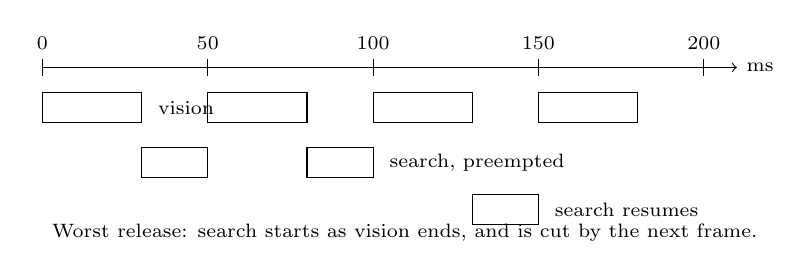
\begin{tikzpicture}[x=0.42mm,y=7mm,font=\scriptsize]
\draw[->] (0,3) -- (210,3) node[right] {ms};
\foreach \x/\lab in {0/0,50/50,100/100,150/150,200/200} {
  \draw (\x,2.85) -- (\x,3.15);
  \node[above] at (\x,3.15) {\lab};
}
\draw (0,2) rectangle (30,2.55);
\node[anchor=west] at (32,2.27) {vision};
\draw (50,2) rectangle (80,2.55);
\draw (100,2) rectangle (130,2.55);
\draw (150,2) rectangle (180,2.55);
\draw (30,1) rectangle (50,1.55);
\draw (80,1) rectangle (100,1.55);
\node[anchor=west] at (102,1.27) {search, preempted};
\draw (130,0.15) rectangle (150,0.7);
\node[anchor=west] at (152,0.42) {search resumes};
\node[anchor=west] at (0,0) {Worst release: search starts as vision ends, and is cut by the next frame.};
\end{tikzpicture}
\caption{Worst-case phasing used for the 70~ms response bound. Vision (top) preempts the factor search (bottom). The search still finishes inside the 200~ms deadline.}
\label{fig:schedule}
\end{figure}

\subsection{A slice of the cost grid}

The search is small enough that a slice of it can be printed. Table~\ref{tab:grid} evaluates Equation~\eqref{eq:cost} at the nominal red-oak diameter 20.5~mm with coefficient of variation 0.15, terrain frequency 6~Hz, slip 0.02, vision flag 0, and the predictor's terrain weight. The predictor does not use $\alpha_{\mathrm{iso}}=0.55$. It uses
\begin{equation}
f_{\mathrm{eff}} = \sqrt{0.35\,f_{\mathrm{dist}}^2 + f^2},
\label{eq:feffpred}
\end{equation}
which is a terrain coefficient $\sqrt{0.35}\approx 0.59$, slightly more pessimistic than the plant coefficient 0.55. The pessimism is intentional in the script that produces Chapter~\ref{ch:estimate}: the search plans for a worse mount than the plant applies. The difference is small. It is recorded here so that a reader who recomputes $f_{\mathrm{eff}}$ with 0.55 and does not match a grid point knows which constant moved.

\begin{table}[htbp]
\centering
\caption{Predicted cost $J$ for nominal red oak at a 6~Hz terrain frequency. Lower is better. Vacuum is in kPa and frequency in Hz.}
\label{tab:grid}
\begin{tabular}{@{}lrrrrr@{}}
\toprule
$f$ & $P=0$ & $P=1$ & $P=2$ & $P=3.5$ & $P=5$ \\
\midrule
3 & 3.052 & 3.157 & 3.267 & 3.443 & 3.631 \\
6 & 2.844 & 2.942 & 3.046 & 3.213 & 3.394 \\
9 & 2.171 & 2.255 & 2.346 & 2.494 & 2.657 \\
12 & 3.219 & 3.300 & 3.387 & 3.529 & 3.685 \\
\bottomrule
\end{tabular}
\end{table}

Every row prefers $P=0$. The vacuum term in Equation~\eqref{eq:zd} has no benefit at $\nu=0$ for this diameter, and the price 0.01 per kilopascal makes a useless vacuum strictly worse. The best printed point is 9~Hz and 0~kPa, with $J=2.171$. Twelve hertz is worse than 3~Hz because $f_{\mathrm{eff}}$ crosses the 10~Hz anchor: $\sqrt{0.35\cdot 36+144}=\sqrt{156.6}=12.5$~Hz. Nine hertz stays under it: $\sqrt{0.35\cdot 36+81}=9.59$~Hz. The Monte Carlo runs select this same corner for mild red oak, so the printed slice and the long runs agree on the nominal lot.

The harsh slice is a near-tie, and the thesis should say so rather than invent a wide margin. At $f_{\mathrm{dist}}=16$~Hz and $P=0$, the same nominal diameter gives $J(3)=3.052$ and $J(9)=3.052$, equal to three digits, with 9~Hz lower only in the fourth digit ($3.0521$ against $3.0522$). Four hertz and 8~Hz are worse, near 3.10 and 3.12. The agitation credit of sitting on $f^{\star}\approx 9.85$~Hz almost cancels the harshness of pushing $f_{\mathrm{eff}}$ to about 13~Hz. The recorded harsh-case run in Chapter~\ref{ch:estimate} selected 3~Hz because the search sees the sample mean of the drawn diameters, not the nominal 20.5~mm, and because a tie keeps the earlier grid point only when the later point is not strictly smaller. A sample mean a few tenths of a millimetre off nominal is enough to break a tie this close. The design consequence is practical. Under a 16~Hz disturbance the coordinator does not have a deep preference between a quiet command and the preferred agitation. Both beat the middle frequencies. A later bench that measures a true preference should replace the harshness coefficient before anyone treats 3~Hz as a unique optimum.

\subsection{Actuator lag and the slew limit}

The grid writes a step. The shaker and the regulator do not. Each is modelled, for the purpose of the slew numbers only, as a first-order lag
\begin{equation}
\tau_a \dot f_a + f_a = f, \qquad \tau_a \dot P_a + P_a = P,
\label{eq:lag}
\end{equation}
with $\tau_a\le 40$~ms so that a 2~Hz step is 95 percent complete in about 120~ms and a 1~kPa step likewise. The requirement stated in the stacking list was 150~ms. The lag model shows that the requirement is a time-constant requirement of about 40~ms, not a vague ``fast enough''. A shaker amplifier that is fast in current and slow in mechanical stroke will violate it even if the electrical specification looks fine. The stroke is the quantity in Equation~\eqref{eq:feff}.

The slew limit of 2~Hz per 200~ms step is 10~Hz per second, which a 40~ms lag can follow. The limit is therefore not hiding an actuator that cannot keep up. It is preventing the search from chattering between the 3~Hz and 9~Hz near-tie when the sample mean jitters. Without the slew, a mean that wanders by a tenth of a millimetre would bang the shaker between two equally good commands. With the slew, a change from 9~Hz to 3~Hz takes three periods, 0.6~s, which is about two or three cell events at 4.4~seeds/s. The seeds in between see an intermediate frequency. That intermediate is one of the middle frequencies the grid dislikes. The estimation does not simulate the slew. It applies the chosen command for the whole run, because each reported case has constant lot statistics and a constant disturbance. A bout in which the disturbance steps from 6~Hz to 16~Hz would pay a short transient the tables do not contain. The transient is bounded by 0.6~s of travel, about 0.7~m at 1.1~m/s, which is three target spacings. Three spacings are visible on a belt and invisible in a 4{,}000-event mean.

\subsection{Failure modes of the stack}

Table~\ref{tab:fmea} lists the failures that change a command, the detection that is actually implemented by the rules already stated, and the command that remains. A failure with no detection does not belong in a table that pretends to be an analysis. Those failures are listed as undetected on purpose.

\begin{table}[htbp]
\centering
\caption{Failures, the detection the design really has, and the command that remains.}
\label{tab:fmea}
\begin{tabular}{@{}p{32mm}p{38mm}p{62mm}@{}}
\toprule
Failure & Detection & Command that remains \\
\midrule
Late vision frame & Datagram age & Last $B$, then decay after 150~ms \\
Wrong scale factor in the camera & Not detected online & A biased $B$. Caught only by the disk calibration \\
Shaft encoder stop & Two missed periods & Motor current removed \\
Radar stuck at a high speed & Not detected online & $\omega^{\star}$ follows the stuck value. A separate timeout on acceleration would be a revision \\
Late factor search & Deadline at 200~ms & Previous $(f,P)$ \\
Search and plant disagree on $\alpha$ & Not a failure. The 0.35 weight is specified & Search is pessimistic relative to the plant \\
Vacuum transducer offset & Zero check at start only & A drifting offset reintroduces doubles. No in-bout zero \\
Depth potentiometer bias & Rail calibration only & A constant depth bias. Spacing scatter grows through $\varepsilon_h$ \\
Isolator collapse, $\alpha\to 1$ & Only if $f_{\mathrm{dist}}$ on the frame rises and the search reacts & The search sees the harsher frequency and moves $f$ \\
\bottomrule
\end{tabular}
\end{table}

Two rows deserve a longer remark because they are the ones a demonstration could hide. A stuck radar is worse than a dead radar. The dead case is specified: after 200~ms the command is held and then ramped to zero. A stuck high case looks like a healthy sensor that believes the tractor is moving. Seeds are metered onto a machine that is standing still, which piles wooden seeds in one spot. The design as written does not detect this. A revision that compares radar speed with the undriven-wheel encoder, and trips when they disagree by more than 15 percent for half a second, would close it. The revision is named here so that the gap is part of the design record rather than a surprise on the first stationary test.

A camera scale error is the other silent fault. The bridge index moves when the millimetre scale moves, because oversize in Equation~\eqref{eq:bridge} is a ratio of diameters. A scale that reads 10 percent high makes a 22~mm seed look like a 24~mm seed and under-calls the bridge. The disk calibration catches a scale error at service. Nothing catches it after the camera is knocked. A cheap in-bout check is the diameter implied by the tube-gate pulse width, which depends on seed size and not on the camera. The design logs the pulse width and does not compare it. The comparison is a consistent extension of the ``tube gate is a logger'' rule: the logger can audit the camera without entering the constraint. Putting the pulse width inside $B$ would couple a post-release sensor into a pre-release decision and would reintroduce the delay the cascade was built to avoid.

\subsection{Quantization, one cell period, and a two-step horizon}

The shaft encoder sets a floor under the fuzzy loop that the continuous model hides. A 4096-count encoder on the cell shaft has an angular quantum of $2\pi/4096=1.53\times 10^{-3}$~rad. At the 10~ms sample the corresponding speed quantum, if speed is a first difference, is $0.153$~rad/s. The nominal red-oak command is $2.30$~rad/s, so the quantum is 6.7 percent of the command if the difference is taken raw. That is coarser than the 0.012 tracking residual used in the estimation, and it would dominate the fuzzy input $\widetilde{\Delta e}$. The feed computer therefore does not differentiate adjacent samples alone. It fits speed over a window of $N_w=8$ samples, 80~ms, which divides the quantum by 8 and yields a speed quantum of about $0.019$~rad/s, just above the residual and just below the scale of $\Delta e$ that moves a membership from zero to small. Eighty milliseconds is 0.44 of the motor time constant, so the window adds lag of that order. The derivative filter of Equation~\eqref{eq:dfilt} and the window are redundant if both are naive. The specification is that the windowed speed is the feedback $\omega_n$, and the derivative filter runs on the tracking error of that already-windowed speed. A second difference of the raw counts is not computed.

The same 80~ms window is the right size relative to a cell. At $\omega=2.30$~rad/s a 12-cell wheel presents a new cell every $2\pi/(12\omega)=0.228$~s. The vision period, 50~ms, samples the throat about four times per cell. The motor period samples it about 23 times. The factor period, 200~ms, is almost one cell. A constraint that changes $\sigma$ therefore takes effect on the cell that is about to be filled, not on a cell that has already released. This timing is the reason the camera looks at the throat rather than at the tube. A tube gate 0.3~s later, from the flight calculation, reports a cell that the wheel has already left. Four vision samples per cell is also the budget inside which a single aborted frame, the 30~ms abort of the response-time argument, still leaves three frames. The bridge index is a vote across those frames through the one-pole filter of Equation~\eqref{eq:rhofilter}, whose 0.92 coefficient remembers roughly twelve frames. A one-frame lie decays. A real bridge, present for a third of a second, accumulates.

A two-step horizon is the natural objection to the one-step grid. Suppose the disturbance is known to step from 6~Hz to 16~Hz one period from now, and the command is 9~Hz. A two-step search could move toward 3~Hz on this period, arriving as the step arrives, whereas the one-step search waits to see 16~Hz and then slews. The value of that preview is the cost of three spacings of intermediate frequency, which the slew analysis already bounded at about 0.7~m of travel. Preview would save that 0.7~m. It would require a forecast of terrain frequency. The inertial unit's one-second Fourier window is a report of the past second, not a forecast of the next 200~ms. Using it as a forecast would be a model of the ground that this machine does not have. The one-step search is the controller that matches the sensor. A terrain map from a previous pass would justify a two-step, or a longer, horizon, and would be a different study, closer to the prescription maps of variable-rate cereal planting than to a single-row hardwood meter \cite{stafford2000,gebbers2010,liu2025review}.

The small-gain view of the constraint is similar in spirit. The map from $\sigma$ to the next bridge index is not known as a transfer function. What is known is a bound. The scale cannot fall by more than 0.22, and the occupancy filter cannot move by more than 0.08 of its input per vision sample. A scale cut therefore cannot chase its own tail inside one cell period: the wheel slows, the filter moves a small step toward the clear-throat target, and the next $\sigma$ is computed from a $B$ that has not yet fully forgotten the bridge. The loop can oscillate only if $B$ itself oscillates, which a real arch does not do at 20~Hz. The cap and the filter are the small-gain ingredients. They are not a computed gain margin. They are the structural reason a margin is plausible, and they are the knobs a bench would turn if the wheel hunted.

\subsection{Rates and power a builder can check with a stopwatch}

The kinematic numbers are simple enough to audit without the simulator, and they should be audited, because every later index is a fraction of them. At $v=1.10$~m/s and $X_t=0.25$~m the target is $\lambda^{\star}=4.40$~seeds/s, which is 264~seeds per minute and 15{,}840~seeds per hour. A 15~litre hopper holding acorns at a bulk density near 0.6~kg/L holds about 9~kg. Red-oak acorns near 4.6~g give roughly 2{,}000~seeds in a full hopper, which is $2000/4.40\approx 455$~s, or seven and a half minutes, of continuous metering. The hopper is a short-bout vessel on purpose. A refill warning at 15 percent mass fires with a little more than a minute left, which is enough to stop at the end of a pass and not enough to forget. Pin-oak seeds are lighter, so the same mass is more seeds and a longer bout. Bur oak is the opposite. The warning is on mass, not on a seed count, because the load cell does not know the species and the camera's count of the throat is not a count of the hopper.

The shaft speed that serves this rate, with twelve cells and a unit fill, is 22.0~r/min. A builder with a tachometer and an empty throat can command that speed and watch the encoder. The check does not need seeds. If the tachometer reads 22~r/min while the radar reads 1.10~m/s and the set spacing is 0.25~m, Equation~\eqref{eq:wstar2} is implemented. Seeds are what test the fill, not the arithmetic.

The energy proxy can be audited in the same spirit. The script accumulates $0.08\omega^2+0.012 f^2+0.02 P^2$ once per cell event. At the mild red-oak both-mode point, $\omega=2.30$~rad/s, $f=9$~Hz, and $P=0$, one event costs
\begin{equation}
0.08\cdot(2.30)^2 + 0.012\cdot 9^2 + 0 = 0.423 + 0.972 = 1.395,
\end{equation}
which matches the table entry 1.39. The shaker term is 70 percent of the proxy. At the harsh-case command $f=3$~Hz the shaker term falls to $0.012\cdot 3^{2}=0.108$, and the wheel term is unchanged, so the event cost falls near $0.53$, again the order of the harsh-case table. The proxy is not a wattmeter. It is a weighted sum that makes this comparison obvious: the camera and the fuzzy increments do not appear in it, and the shaker does. A builder who later measures current will not reproduce 1.39. A builder who finds that the shaker current is a small fraction of the wheel-motor current has discovered that the prices in $J$ were in the wrong ratio, and should raise the frequency price or lower the wheel weight before trusting the quiet-versus-loud tie. The functional form is the part worth keeping. The coefficients 0.08, 0.012, and 0.02 are placeholders until a current clamp replaces them.

Cell time and computer time meet in one inequality that is worth writing as a release check. A cell period is 0.228~s at the nominal rate. Inside that period the feed computer runs about 23 motor steps, the vision computer owes four frames, and the factor computer owes one search. The sums of the budgets are $23\times 2$~ms, $4\times 30$~ms, and 40~ms, which are 46~ms, 120~ms, and 40~ms. The vision budget sum, 120~ms, fits in 228~ms with 108~ms to spare, but only if the four frames do not stack. They do not stack if each frame is aborted at 30~ms, because $4\times 30=120<228$ and the frames are released 50~ms apart. The inequality $4\times 30~\mathrm{ms}<0.228~\mathrm{s}$ is the release check for the nominal speed. It fails at a shaft speed high enough that the cell period drops below 120~ms, which would be $\omega>2\pi/(12\cdot 0.120)=4.36$~rad/s, or about 42~r/min, corresponding to $v=2.08$~m/s at this spacing. The machine is not specified to run there. The inequality says why. It is the same lesson as the 6~km/h reversal on the corn meter, written as a speed limit that belongs to the vision budget rather than to the agronomy \cite{borja2021}.

\subsection{What an empty cell does to the count}

The rate audit above assumes every cell releases one seed. The indices exist because that assumption fails, and the failure has a counting form that is easy to misread on a display. Suppose that over $N$ cell passages the machine travels $N X_t/\sigma$ and releases $N_s$ singles and $N_d$ doubles, with the rest empty. The number of seeds is $N_s+2N_d$. The number of positive spacings is one less than the number of seeds, which for a long run is essentially $N_s+2N_d$. A double contributes a short spacing and also splits what would have been one interval into two, so it increases the spacing count. A miss contributes no spacing of its own. It lengthens a neighbour. The miss index is therefore not $100(N-N_s-N_d)/N$. That ratio is the empty-cell rate. The miss index is the fraction of observed spacings that exceed $1.5X_t$. If empties arrive in isolation, each empty lengthens one spacing from about $X_t$ to about $2X_t$ and the miss index is close to the empty-cell rate. If two empties arrive together, one spacing of about $3X_t$ replaces two empty cells in the count, and the miss index, which divides by the number of spacings rather than by the number of cells, moves differently from the empty-cell rate. The plantation looks worse. The percentage may rise or fall. The estimation's event model places isolated empties more often than bursts, because each event is drawn independently. A real arch lasts for several cells and would burst. The bridge constraint is the mechanism aimed at that burst: it slows the wheel while $B$ stays high, which is a run of cells rather than one draw. The independent-draw estimation therefore understates the value of the constraint on true arches and overstates the chance that a single slow cell is enough. That bias is a reason the both-mode gain on bur oak in Chapter~\ref{ch:estimate} should be read as a lower bound on what a persistent bridge would give the constraint to do, and as an upper bound on how tidy the resulting spacings would look. Independent draws make tidy tables. Arches make clumps. The controller is designed for the clumps. The table is computed from the draws. Both facts belong in the design record so that a belt test full of clumps is not scored as a refutation of a table that assumed none.

A twenty-cell strip makes the distinction numerical. Write E for an empty cell and S for a single, and ignore doubles. The release pattern
\[
\mathrm{S\,S\,E\,S\,S\,S\,E\,E\,S\,S\,S\,S\,E\,S\,S\,S\,S\,S\,E\,S}
\]
has five empties in twenty cells, an empty-cell rate of 25 percent. The spacings, in units of $X_t$ and dropping the final open end, are approximately
\[
1,\,2,\,1,\,1,\,3,\,1,\,1,\,1,\,2,\,1,\,1,\,1,\,1,\,2.
\]
Fourteen spacings follow. Four of them exceed $1.5$, so the miss index is $4/14\approx 29$ percent, against an empty-cell rate of 25 percent. The denominator shrank, because an empty cell does not create a spacing of its own, and the double empty became one spacing of 3 rather than two entries. A display that shows 25 percent skips from the tube gate, which counts empties, and a display that shows 29 percent miss index from a belt, which counts spacings, are both right. They are not the same statistic. The estimation reports the belt statistic, Equations~\eqref{eq:imult}--\eqref{eq:imiss}. The tube gate in the build reports the empty-cell rate through Equation~\eqref{eq:etahat}. An operator who treats them as one number will ``tune'' a controller that is already consistent. The design keeps them on different computers for that reason, not only for the deadline.

\subsection{What the extra analysis changes}

None of these calculations change the five modes of the estimation. They change what a disagreement with the estimation would mean. A two-centimetre bias is flight, not a bad gain. A tie between 3~Hz and 9~Hz is a flat cost, not a bug in the arg-minimum. A vision overrun that is allowed to finish is a broken response-time bound, not a mysterious rise in misses. The controllers remain the constraint of Equation~\eqref{eq:sigma} and the grid of Equation~\eqref{eq:cost}. The surrounding arithmetic is the part that makes those two equations implementable on the two computers of Section~\ref{sec:build} without confusing their faults with their tuning.

